\documentclass[a4paper]{article}
\usepackage{german}
\usepackage[utf8]{inputenc}

\usepackage{pgfplots}

\usepgfplotslibrary{groupplots}

\begin{document}

\begin{center}
\dotfill
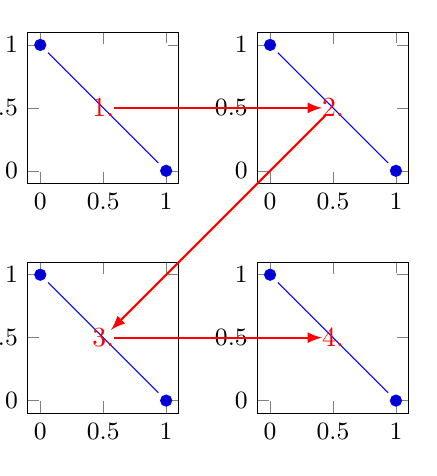
\begin{tikzpicture}[shorten >=4pt,shorten <=4pt,
	%trim left={(group c1r1.south west)},trim axis right,
	trim axis group left,
	trim axis group right,
	]
  \begin{groupplot}[group style={group size=2 by 2},
    height=3.5cm,width=3.5cm,/tikz/font=\small]
    \nextgroupplot% 1
    \addplot coordinates {(0,1) (1,0)};
    \nextgroupplot% 2
    \addplot coordinates {(0,1) (1,0)};
    \nextgroupplot% 3
    \addplot coordinates {(0,1) (1,0)};
    \nextgroupplot% 4
    \addplot coordinates {(0,1) (1,0)};
  \end{groupplot}
  \draw[thick,>=latex,->,red]
    (group c1r1.center) node {1.} --
    (group c2r1.center) node {2.};
  \draw[thick,>=latex,->,red]
    (group c2r1.center) --
    (group c1r2.center) node {3.};
  \draw[thick,>=latex,->,red]
    (group c1r2.center) --
    (group c2r2.center) node {4.};
\end{tikzpicture}%
\dotfill
\end{center}

\end{document}

